\documentclass[]{scrartcl}
\usepackage{graphicx}
\usepackage{caption}
\usepackage{geometry}
\usepackage{authblk}
\usepackage{subcaption}
\usepackage{amsmath}
\renewcommand{\thefigure}{S\arabic{figure}}

\newgeometry{top=3cm,bottom=3cm,left=3cm,right=3cm}

\title{Supplementary Material \\
	{\normalfont Genome-wide pre-miRNA discovery from few labeled examples}}
\date{}
\author{C. Yones, G. Stegmayer and D. H. Milone}
\affil{\small  Research Institute for Signals, Systems and Computational Intelligence, sinc(\textit{i}), FICH-UNL, CONICET, Santa Fe, Argentina.}

\begin{document}

\setcounter{page}{89}
\maketitle

\section*{Supplementary Figure S1: parameters sensitivity test}
	\begin{figure}[h!]
		\centering
		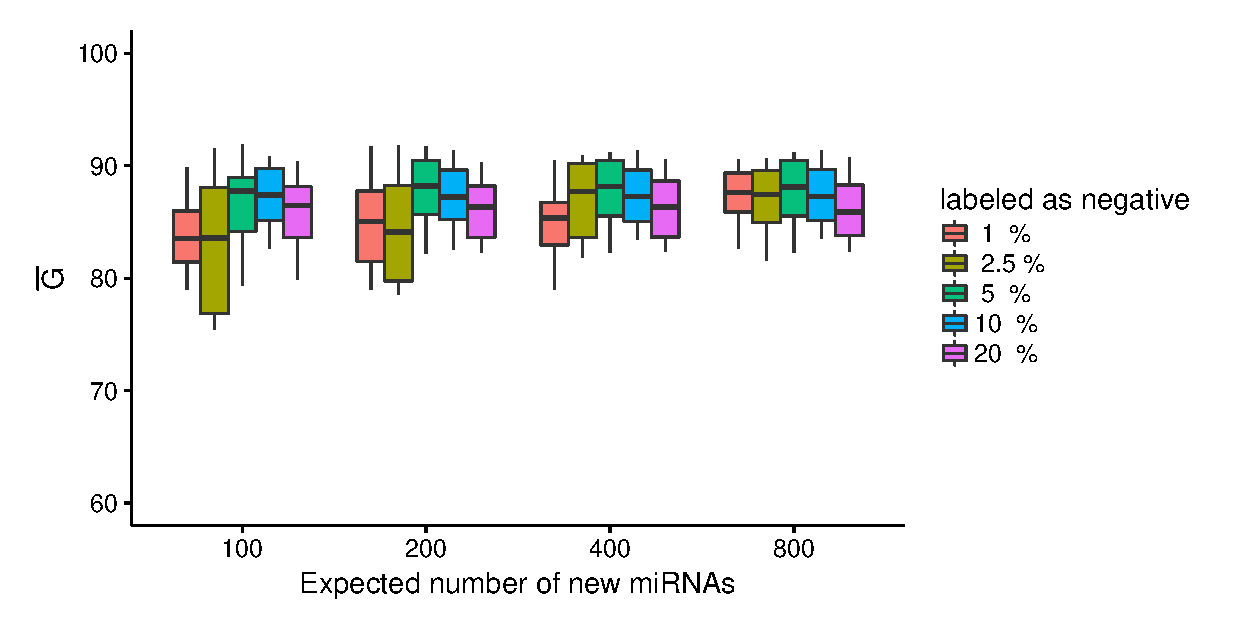
\includegraphics[width=\textwidth]{resources/sensitivity_test.eps}
		\label{fig:sensitivity_test}
	\end{figure}
	In this experiment, 20 combinations of the expected number of pre-miRNA to be find and the percentage of hairpins that will be labeled as negative examples to initiate the prediction algorithm have been tested on a cross-validation scheme, with the genome-wide dataset of \textit{C. elegans}. The real number of true pre-miRNAs is 249, but as can be seen, for any estimation between 100 and 800 miRNAss maintains a good and stable performance. The same happens with the percentage of negative examples automatically labeled.

\newpage
\section*{Supplementary Section S2: avoiding misclassification of labeled examples}

	To avoid the misclassification of positive examples, the constant $c$ must be large enough to ensure that any misclassification of positive examples would yield a greater penalization than the regularizing term of the objective function. This value can be estimated from the equations of the method. Given the definition
	\begin{equation} \tag{S.1}
		a_{ij} =
		\begin{cases}
			\frac{\mu}{\mu + ||\mathbf{x}_{i} - \mathbf{x}_{j}||^2} & \text{if} \ \mathbf{x}_{j} \in  \mathcal{K}(\mathbf{x}_{i}) \ \text{and} \ \ell_{i} \ell_{j} \geq 0 \\
			0 & \text{in other cases,} \\
		\end{cases}
	\end{equation}

	\noindent since the norm cannot be negative, then $a_{ij} \leq 1$. Therefore, $d_{ii} = \sum_{k=0}^n a_{ik} \leq k$. From (2) in the manuscript,

	\begin{equation} \tag{S.2}
		\begin{split}
			\mathbf{z}^T L \mathbf{z} & = \mathbf{z}^T I \mathbf{z} - \mathbf{z}^T {D^{-1/2}}^T A D^{-1/2} \mathbf{z} \\
			& = \sum_{i}^{n} z_{i}^{2} -  \sum_{i}^{n}  \sum_{j}^{n} \frac{z_{i}}{\sqrt{d_{ii}}} \frac{z_{j}}{\sqrt{d_{jj}}} a_{ij} \\
			& = n -  \sum_{i}^{n}  \sum_{j}^{n} z_{i} z_{j} \frac{a_{ij}}{\sqrt{d_{ii}} \sqrt{d_{jj}}}   \\
			& \leq n -  \sum_{i}^{n}  \sum_{j}^{n} z_{i} z_{j} \frac{1}{k}   \\
			& = n -  \sum_{i}^{n} \frac{z_{i}}{k} \sum_{j}^{n}  z_{j} =  n -  \sum_{i}^{n} \frac{z_{i}}{k} 0 = n \\
		\end{split}
	\end{equation}

	\noindent Then, the misclassification of a positive example must have a penalization greater than $n$. A positive example $\mathbf{x}_{i}$ is misclassified when $z_{i} \leq 0$, which leads to
	\begin{equation} \tag{S.3}
		c (z_{i} - \ell_{i}) C_{ii} (z_{i} - \ell_{i}) \geq c (0 - \ell_{i}) C_{ii} (0 - \ell_{i}) = c \gamma_{+} C_{ii} \gamma_{+} .
	\end{equation}
	\noindent Then, to avoid the misclassification
	\begin{equation} \label{eq:ineq} \tag{S.4}
		\begin{split}
			c \gamma_{+} C_{ii} \gamma_{+} & > n \\
			c \sqrt{\frac{n_{-}}{n_{+}}} C_{ii} \sqrt{\frac{n_{-}}{n_{+}}} & > n \\
			c \frac{n_{-}}{n_{+}} C_{ii} & > n \\
			c C_{ii} & > \frac{n_{+} n}{n_{-}} \\
		\end{split}
	\end{equation}

	\noindent Therefore, any combination of $c$ and $C_{ii}$ that fulfills the inequality \ref{eq:ineq} would avoid the misclassification of positive examples. One option is to leave $C_{ii}=1$ as default, and set $c > \frac{n_{+} n}{n_{-}}$. This parameter has the disadvantage that it also modifies the penalization for the negative examples. Another better solution is to leave $c = 1$ as default, and set $C_{ii} > \frac{n_{+} n}{n_{-}}$ for the positive examples. With this setting only the positive examples are protected from misclassification.

\newpage
\section*{Supplementary Figure S3: thresholding the prediction scores}
	\vspace{4pt}
	\begin{figure}[h!]
	\centering
		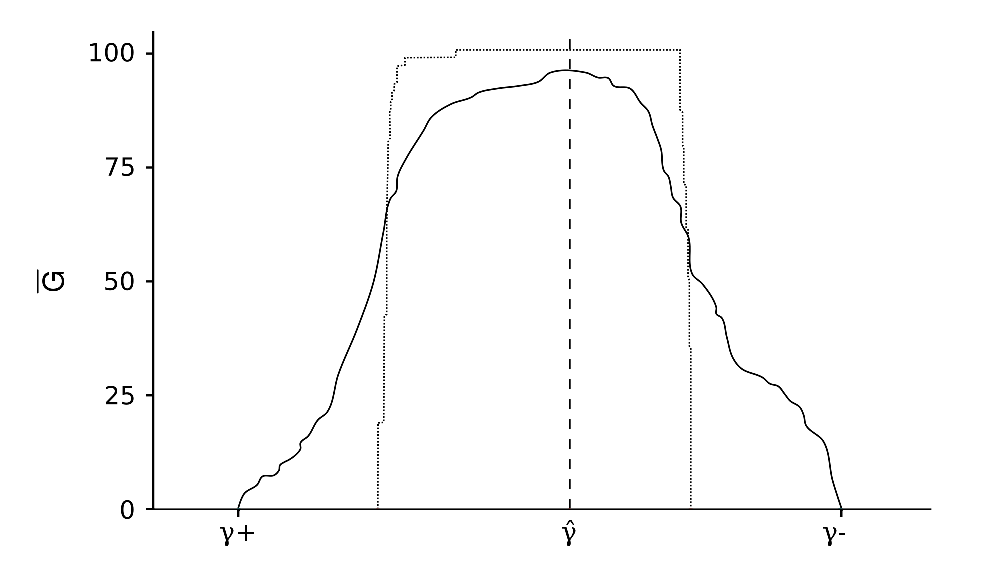
\includegraphics[width=0.8\textwidth]{resources/threshold.eps}
		\label{fig:threshold}
	\end{figure}
	\vspace{4pt}

	Comparison of the estimated (dotted line) and the real (solid line) geometric mean ($\bar{G}$) of sensitivity and specificity in an example dataset. Between two consecutive labeled samples in $\mathbf{z}^\star$ increasingly sorted by $\bar{G}$, there could be many unlabeled sequences. Hence, the estimated performance measure remains constant in those regions. When the number of labeled samples is low, this regions can be quite wide, therefore the final threshold ($\hat{\gamma}$) is set as the midpoint between the highest and the lowest scores in $\mathbf{z}^\star$ which maximizes the performance measure.

\newpage
\section*{Supplementary Section S4: feature sets}

\vspace{10pt}
{\Large \textbf{Feature set 1 (FS1)}}
\vspace{2pt}

\begin{itemize}
	\item $tri_A$, $tri_U$, $tri_G$, and $tri_C$: frequencies of secondary structure triplets composed of three adjacent nucleotides and the middle nucleotide: "A(((", "U(((", "G(((", and "C(((".
	\item $orf$: the maximal length of the amino acid string without stop codons found in three reading frames.
	\item $loops$: the cumulative size of internal loops found in the secondary structure.
	\item $dm$: a percentage of low complexity regions detected in the sequence using Dustmasker \footnote{Morgulis, A., Gertz, E. M., Schäffer, A. A., \& Agarwala, R. (2006). A fast and symmetric DUST implementation to mask low-complexity DNA sequences. \textit{Journal of Computational Biology}, \textbf{13}(5), 1028-1040.}
	\item $\%C + G$: aggregated proportion of cytosine and guanine on the sequence.
	\item $dG$: Minimum free energy divided by the sequence length.
	\item $dQ$: is calculated as $$\frac{1}{l} \sum_{i<j} p_{ij} \log_2 p_{ij} , $$	where $p_{ij}$ is the probability of pairing of nucleotides $i$ and $j$. This value is calculated with the software RNAfold with -p option. Low values of $dQ$ correspond to distributions dominated by a few bases likely to be matched. These bases are better predicted than those that have multiple alternative states.
	\item $dF$: topological descriptor. For a further description see Gan \textit{et. al.} (1987)
	\footnote{Gan, H. H., Fera, D., Zorn, J., Shiffeldrim, N., Tang, M., Laserson, U., ... \& Schlick, T. (1987). RAG: RNA-As-Graphs database—concepts, analysis, and features. \textit{Nutrition and Health}, \textbf{5}(1-2), 1285-1291.}.

	\item $MFEI_1$: ratio between the minimum free energy and the $\%C + G$.
	\item $MFEI_2$: is calculated as $dG/N_{s}$, where $N_{s}$ is the number of stems.
	\item $MFEI_3$: is calculated as $dG/N_{l}$, where $N_{l}$ is the number of loops in the secondary structure.
	\item $MFEI_4$: is calculated as $MFE/N_{b}$, where $N_{b}$ is the total number of base pairs in the secondary structure.
	\item $zD$: base pair distance for all pair of structures, calculated as $$dD = \frac{1}{l} \sum_{i<j} p_{ij} (1 - p_{ij}) , $$ normalized with z-score.
	\item $Diversity$: the structural diversity calculated with RNAfold (-p option).
	\item $NEFE$: Normalized Ensemble Free Energy calculated with RNAfold (-p option).
	\item $Diff$: is calculated as $|MFE-EFE|/L$.
	\item $dS$: Structure Entropy calculated using UNAfold.
	\item $dS/L$: normalized structure entropy.
	\item $|A-U|/L$, $|G-C|/L$, $|G-U|/L$: number of each possible base pair normalized by the sequence length.
	\item $Avg\_BP\_Stem$: Average of nucleotides per stem.
	\item $\%(A-U)/N_{s}$, $\%(G-C)/N_{s}$ and $\%(G-U)/N_{s}$: proportion of base pairs on stems.
\end{itemize}

\vspace{20pt}

{\Large \textbf{Feature set 2 (FS2)}}
\vspace{2pt}

\begin{itemize}
	\item Nucleotide proportion: ratio of each base in the sequence
	\item Dinucleotide proportion: ratio of dinucleotide elements of each kind.
	\item $L$: sequence length.
	\item $N_{s}$: number of stems.
	\item $\%C + G$: aggregated proportion of cytosine and guanine.
	\item $G/C_{ratio}$: ratio of guanine over cytosine.
	\item $Avg\_BP\_Stem$: average of nucleotides per stem.
	\item Longest stem length: longest region where the pairing is perfect.
	\item Terminal loop length: number of nucleotides in the stem region of the secondary structure.
	\item Number of base pair: number of paired nucleotides divided by 2
	\item $dP$: number of base pair divided by the nucleotide number.
	\item $|A-U|/L$, $|G-C|/L$, $|G-U|/L$: number of each possible base pair normalized by the sequence length.
	\item $\%(A-U)/N_{s}$, $\%(G-C)/N_{s}$ and $\%(G-U)/N_{s}$: proportion of base pairs on stems.
	\item Triplets: Vector of 32 elements with the triplets frequency. A triplet is an element formed with the structure composition (paired or not paired) of three adjacent nucleotides and the base of the middle. An example of these elements is \textquotedblleft.((A\textquotedblright, where the parenthesis represent a paired nucleotide, a dot a not paired one and the letter is the base of the middle nucleotide.
	\item $MFE$: minimum free energy.
	\item $EFE$: ensemble free energy.
	\item $Freq$: the structural frequency calculated with RNAfold (-p option).
	\item $Diversity$: the structural diversity calculated with RNAfold (-p option).
	\item $Diff$: is calculated as $|MFE-EFE|/L$.
	\item $dG$: Minimum free energy divided by the sequence length.
	\item $dQ$: is calculated as $$\frac{1}{l} \sum_{i<j} p_{ij} \log_2 p_{ij} , $$	where $p_{ij}$ is the probability of pairing of nucleotides $i$ and $j$. This value is calculated with the software RNAfold (-p option). Low values of $dQ$ correspond to distributions dominated by a few bases likely to be matched. These bases are better predicted than those that have multiple alternative states.
	\item $MFEI_1$: ratio between the minimum free energy and the $\%C + G$.
	\item $MFEI_2$: is calculated as $dG/N_{s}$, where $N_{l}$ is the number of stems.
	\item $MFEI_4$: is calculated as $MFE/N_{b}$, where $N_{b}$ is the total number of base pairs in the secondary structure.
\end{itemize}

	\newpage
	\section*{Supplementary Figure S5: cross-validation in full labeled datasets}
	%*****************************************************************************************
	\begin{figure}[h]
		\centering
		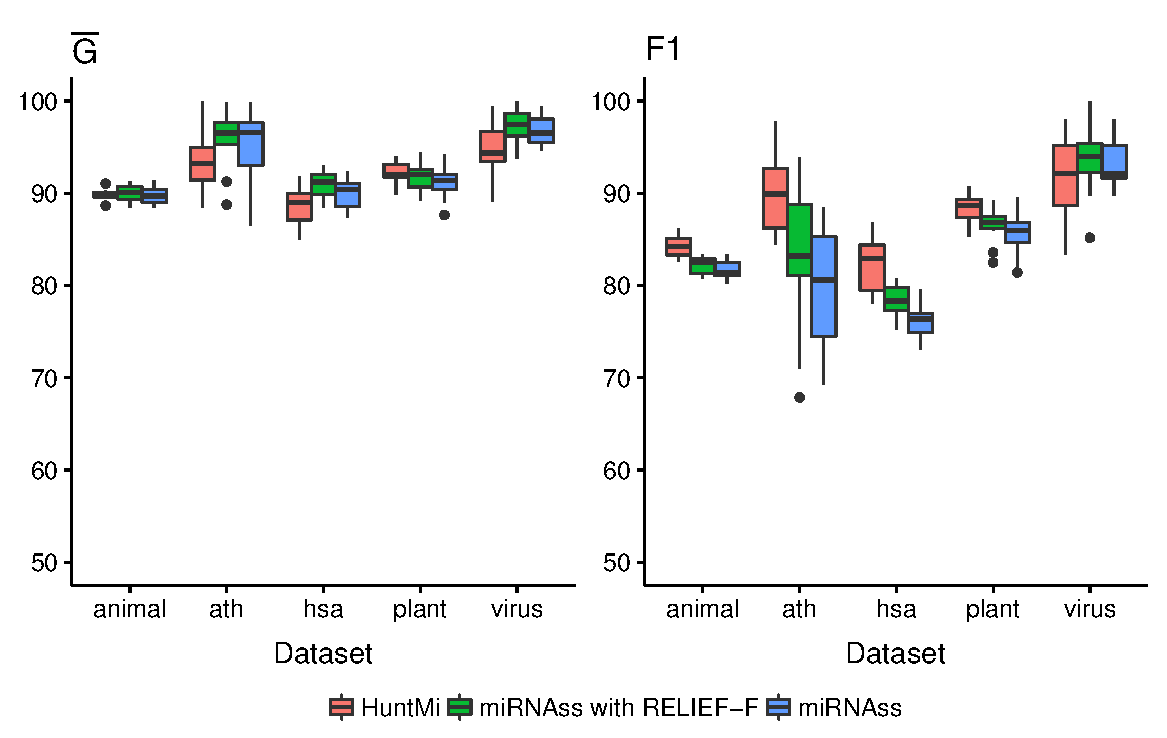
\includegraphics[width=\textwidth]{resources/huntmi_crossvalidation.eps}
		\label{fig:huntmi}
	\end{figure}
	%*****************************************************************************************

	Box plot of $\bar{G}$ and $F_{1}$ obtained by miRNAss and HuntMi in five different datasets. The middle line in each box represents the median of each distribution. The upper whisker extends from the hinge to the highest value, that is, within 1.5 times the interquartile range ($IQR$) of the hinge. The lower whisker extends from the hinge to the lowest value, within 1.5 times $IQR$ of the hinge. Data beyond the end of the whiskers are outliers and are plotted as points.

\newpage
\section*{Supplementary Figure S6: few labeled examples}
	\begin{figure}[h!]
		\centering
		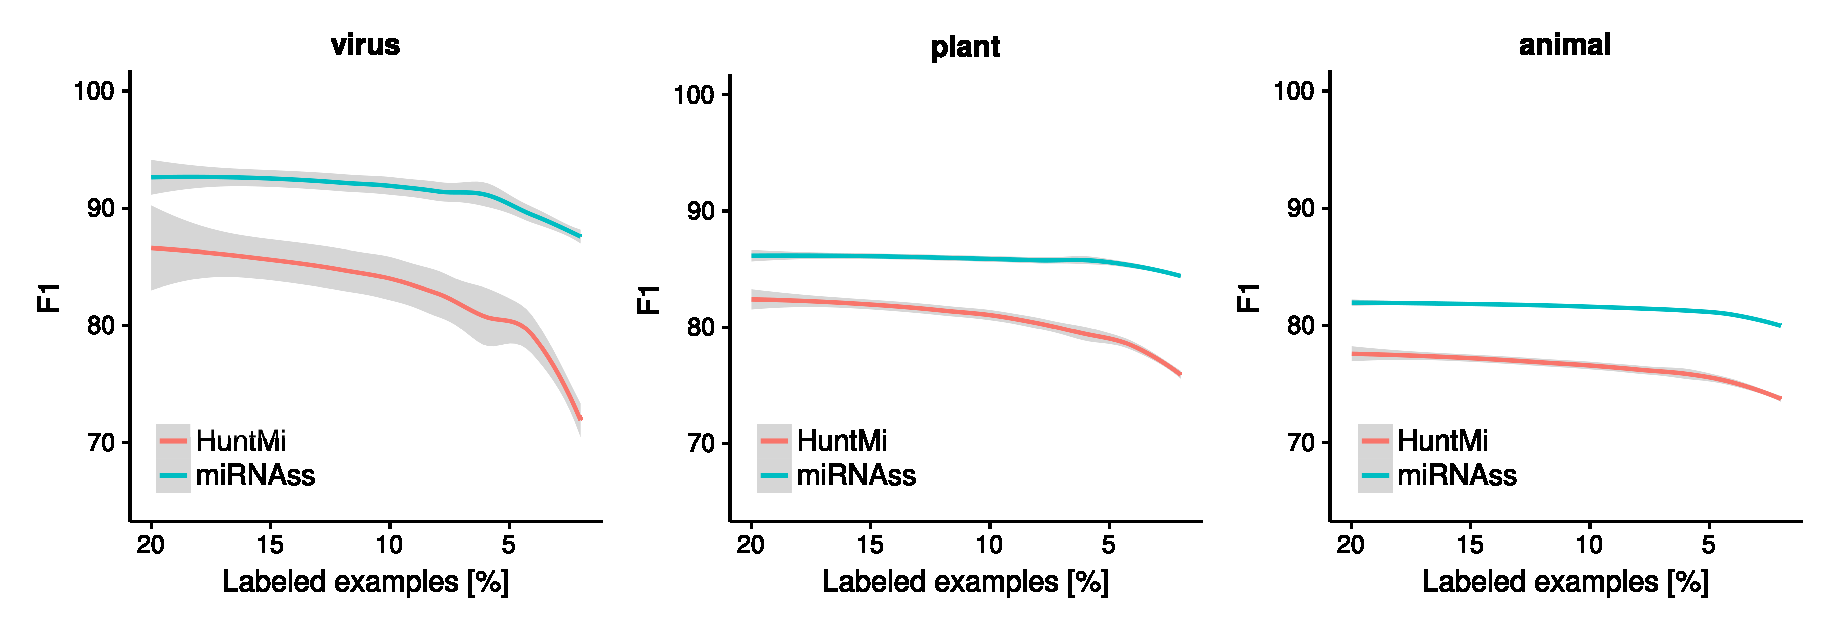
\includegraphics[width=\textwidth]{resources/few_samples_huntmi_all.eps}
		\label{fig:fewSamples}
	\end{figure}

	Curves of $F_{1}$ obtained by decreasing the percentage of labeled sequences. The shaded regions are confidence intervals of the estimation with local regression (LOESS) at $p<0.05$. In the Virus dataset, while the $F_{1}$ achieved by HuntMi falls as the percentage of labeled examples decreases, miRNAss maintains a higher and almost constant $F_{1}$, independently of the percentage of labeled sequences. In the plant dataset, again, miRNAss achieves a higher $F_{1}$ for all percentages; and moreover, this difference increases as the number of labeled examples decreases. In animal dataset, miRNAss maintains an almost constant $F_{1}$ when the percentage of labeled sequences is greater than $5\%$. HuntMi achieves a lower $F_{1}$ for all percentages.

\end{document}
